
\section{Software Architecture}

%{{{
% SECTION: PROGRAMMING LANGUAGES; PLATFORMS AND TOOLS
% [x]  1. Which programming language did you use to implement the multi-agent 
%         system?
% [x]  2. Did you use multi-agent programming languages? Why or why not to use a 
%         multi-agent programming language?
% [ ] Question 3.2 not properly answered. General lack of flexibility: Why? Which languages did you use? Citation?
%    3.2: Did you use multi-agent programming languages? Why or why not to use a multi-agent programming language?

% [x]  4. Which development platforms and tools are used? How much time did you 
%         invest in learning those?
% [x] Question 3.4 not properly answered. Question was more about the question
% what editor did you use for the design process what IDE did you use, what
% about debugger for DeLP, etc. And the hours spent to learn how to use them.
%    3.4: 4. Which development platforms and tools are used? How much time did you invest in learning those?
%            editor for the design process? 
%            what IDE did you use?
%            what abpout debugger for delp?
%            hours spent learning those?
%
%        poner que no usamos IDEs 
%        poner lo del visualizador del arboles dialecticos de delp?

% [x]  5. Which runtime platforms and tools (e.g. Jade, AgentScape, simply Java, 
%         ....) are used? How much time did you invest in learning those?
% [ ]  6. What features were missing in your language choice that would have 
%         facilitated your development task?
% [x]  7. What features of your programming language has simplified your 
%         development task?

% SECTION IMPLEMENTION
% [x]  3. How have you mapped the designed architecture (both multi-agent and 
%         individual agent architectures) to programming codes, i.e., how did 
%         you implement specific agent-oriented concepts and designed artifacts 
%         using the programming language?

% [ ] 10. To which extent is the reasoning of your agents synchronized with the 
%         receive-percepts/send-action cycle?
% [ ] Question 3.10 is not discussed in the paper. Do you do reasoning between two steps?

% [ ] How does the static, dynamic and initial data look like?
% [ ] How does DeLP look like? Only explained later.
% [ ] How does an intention look like?

% [ ]  8. Which algorithms are used/implemented?

% [ ]  9. How did you distribute the agents on several machines? And if you did 
%         not please justify why.

% SECTION: DIFFICULTIES ENCOUNTERED
% [ ] 11. What part of the development was most difficult/complex? What kind of 
%         problems have you found and how are they solved?

% [x] 12. How many lines of code did you write for your software?
% [ ] Question 3.12 not answered.

% This section is a little bit unsorted and too short. I think you should first
% explain the overall structure, then describe each node in detail, i.e., parts
% from 4.2 should go to 4.1.
% Without looking into the source code the reader cannot understand how the agent
% team works, e.g., how do the agents synchronize their intentions?
% In general, a lot of information is missing in order to understand the ideas
% behind the agent team. How do you deal with updates that invalidates old
% information? What about an example? What does the belief base contain? only
% percepts?
% 
%    IÑAKI:
%        como se representa el conocimiento?
%        how does de static dynamic and initial data look like?
%        como se representa entre el agente y el PS?
%        ejemplos de codigo 
%        como se traduce a prolog para meterlo en la KB?
%        UNA BUENA EXPLICACION DEL PIPELINE DE DATOS
%    MANU: how does an intention look like?
%
%    cada turno la informacion en la kb se actualiza, se usa el parametro de step para ver la edad y validez de la info
%    ejemplo el algoritmo de coloreo permite generacion de creencias, por lo cual en la kb no esta solamente la percepcion
%}}}

\subsection{Programming languages, platforms and tools}
    %{{{
    The agent system was implemented using Python 2.7 and SWI Prolog
    5.10.5.  Language integration was achieved using the \textit{pyswip}\
    library\footnote{http://code.google.com/p/pyswip/}, which facilitates the
    execution of Prolog queries from Python.  The implementation of Defeasible
    Logic Programming (DeLP) by the LIDIA \cite{Garcia:2004a} was used for the
    deliberative process, in which desires and intentions are set.  The
    standard Python and SWI-Prolog debugging tools were used.  DeLP includes
    a graphical viewer for dialectical trees, allowing visualization of which
    arguments attack others and facilitating debugging of the defeasible rules
    employed.  
    
    These languages and platforms were well-known at the start of the project,
    and were chosen for precisely those reasons.
    
    No multi-agent programming languages/platforms/frameworks were used due to 
    a lack of familiarity on behalf of the development team. 
    Also, integrating or extending an existing framework with queries to
    defeasible rules was initially considered more difficult than the
    straighforward approach taken.

    Python's amenity to rapid application development and ``batteries-included 
    philosophy'' facilitated implementing the communication layer to the MASSim 
    server, parsing of perceptions, rapid addition of planned features and bug 
    correction. DeLP's capability to deal with conflicting pieces of
    information was also very helpful in order to implement the
    decision-making module. 
    %}}}

\subsection{Implementation}
    %{{{
    The system was implemented as a collection of independent operating system
    processes, the percept server (PS from here onwards) and each agent running
    in its own address space.  The agents are started individually and
    synchronize via the PS.  Each one handles its own connection to
    the MASSim and percep servers, as the \textit{eismassim} package provided
    by the contest organizers was not used to avoid the difficulty of
    integrating yet another language and runtime (Java) with the ones being
    used. 
    
    \begin{figure}
    \centering
    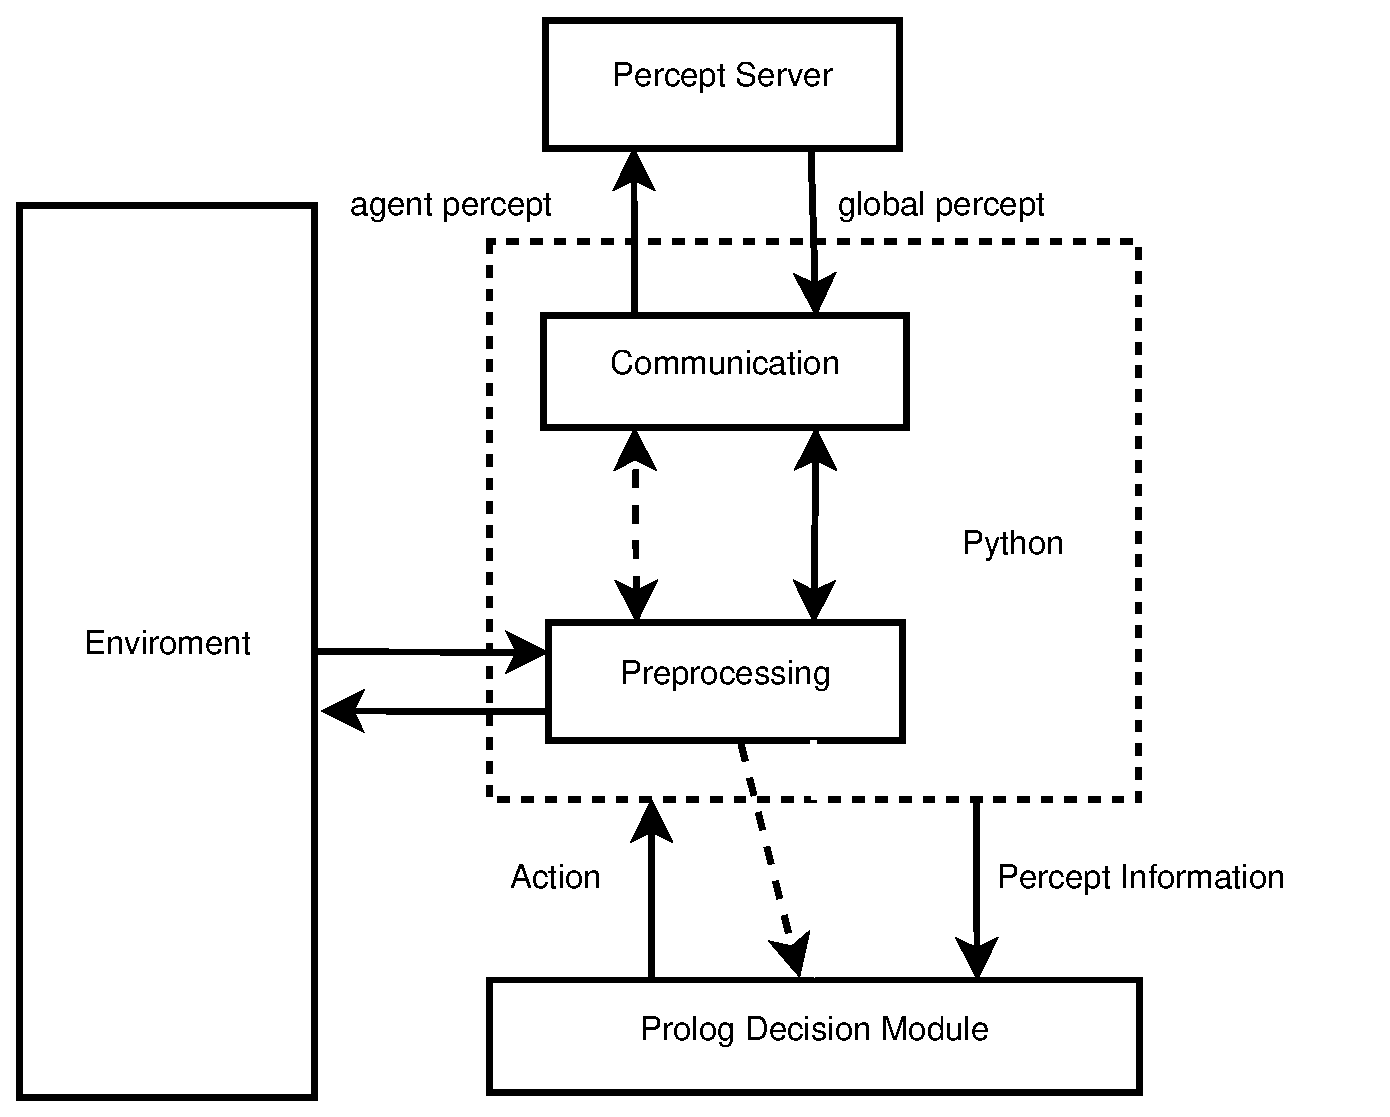
\includegraphics[scale=.3]{agentarchitecture.eps}
    \caption{Agent architecture in a flow chart-like diagram. Dashed arrows
    represent process flow, solid lines represent data flow.}
    \label{fig:architecture}
    \end{figure}

    \begin{figure}[!htb]
    \centering
    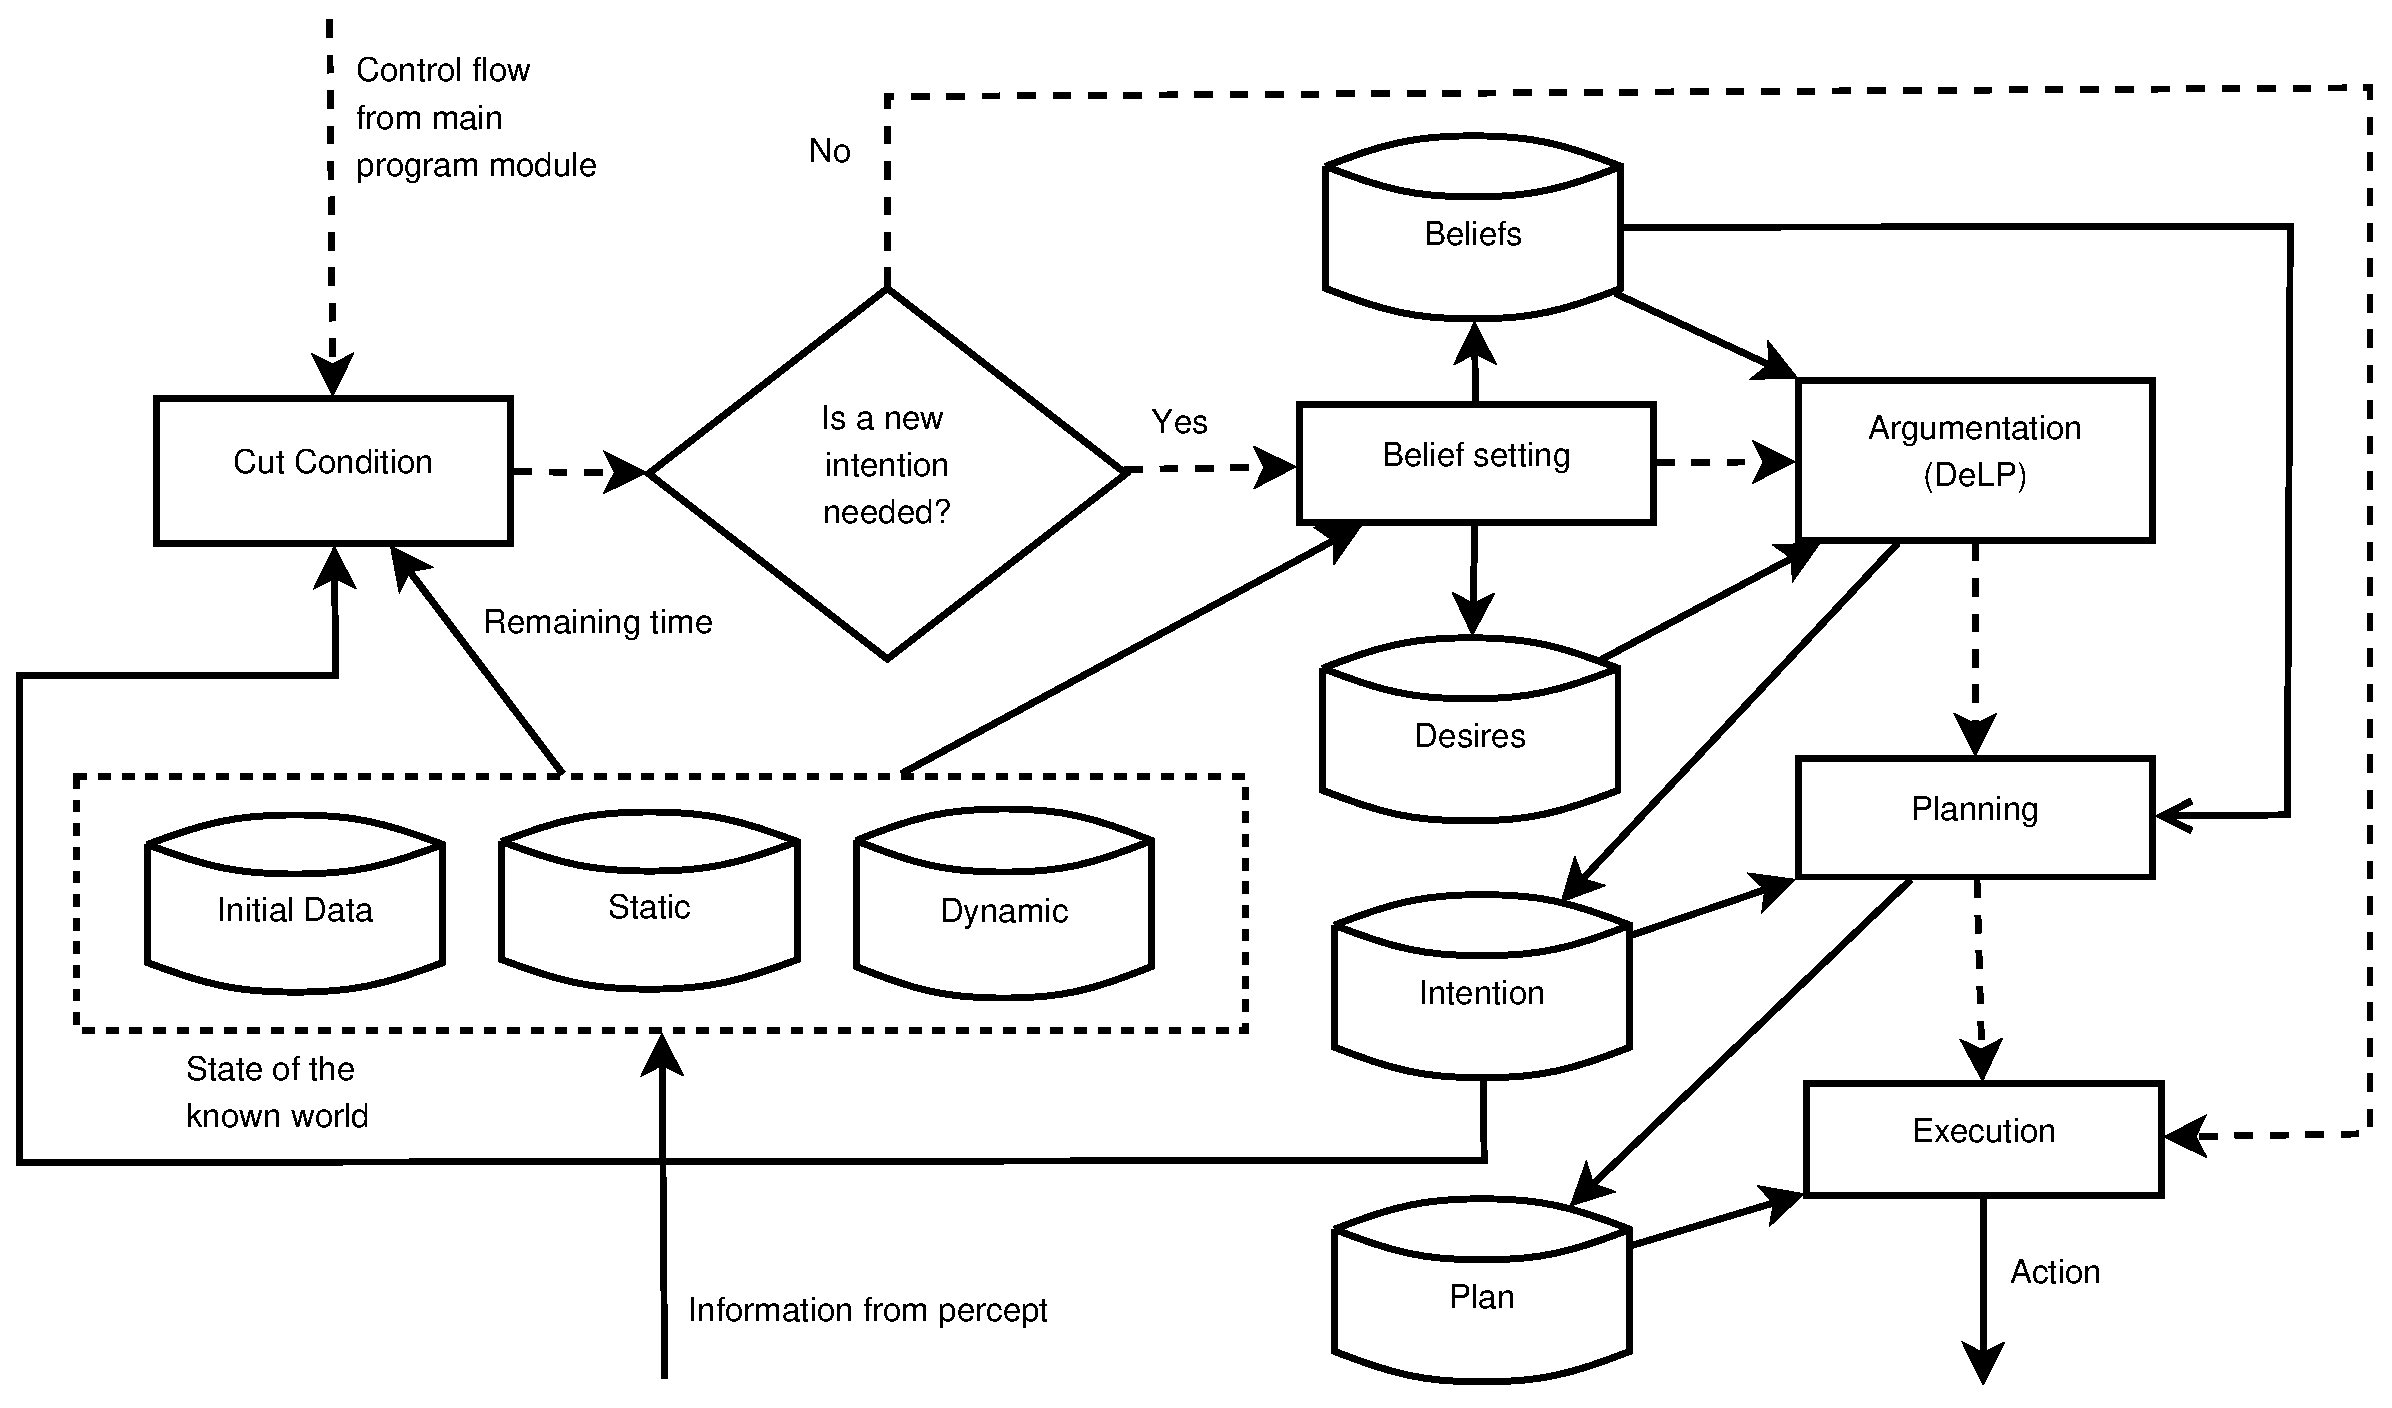
\includegraphics[width=\textwidth]{agentprolog.eps}
    \caption{Architecture of the Prolog decision module}
    \label{fig:prologmodule}
    \end{figure}

    Fig. \ref{fig:prologmodule} shows the structure and flow of control and
    information within the decision making module implemented in Prolog and
    DeLP.
    %}}}
    
\subsubsection{Agent main program.}
    %{{{
    The agent main program is implemented in Python, and handles all
    communication with the servers, XML parsing, processing the information in
    the percept into a form suitable for assertion in the agent's knowledge
    base, and generation of the XML representing the action taken which is
    returned to the MASSim server.

    On startup, an agent is passed the information needed to authenticate with
    the MASSim server and some configuration options such as network addresses
    and ports, whether the PS and the argumentation framework are to
    be used or not, and logging verbosity levels.
    Initialization consists of opening the connections to the MASSim server,
    authenticating, opening the connection to the PS, and starting
    the Prolog engine. The main program loop is then entered, in which messages
    from the MASSim server are received and parsed. 

    When a message of type \texttt{sim-start} is received, initial information
    present in the message such as the agent's role and the simulation
    parameters are asserted into the agent's knowledge base and the perceive-act
    loop is started.

    Each iteration of the perceive-act loop expects a \texttt{request-action}
    message from the MASSim server and parses the XML into a Python dictionary.
    Elements in the percept are divided into a ``public'' section, which is sent
    to the PS to be shared with other team agents and a ``private''
    section.

    If so configured, the agent will then send the percept to the PS and await
    the global percept containing the remainig information perceived by the
    team. The global percept is merged with it's own, and asserted into the
    agent's knowledge base, establishing the agent's beliefs.  Note that no
    information is included in the percept other than what is received in the
    percept.

    The decision making module implemented in Prolog is then queried for the
    next action to be performed by the agent.
    
    Once control flow returns to the Python program with the determined action,
    the corresponding XML message is generated and sent to the MASSim server. 
    %}}}

\subsubsection{Percept Server.}
    %{{{
    The PS maintains a connection for each agent. 
    The connection handling methods encode the associate array into a form
    suitable for conversion into a set datastructure, which is then sent over
    the network. 
    On each iteration, the PS waits for each agent's data, performs a union of
    all data sets, and returns to each agent the set difference between the data
    the agent sent and the total union.

    Figures \ref{fig:pythonperceptpublic} and \ref{fig:pythonperceptprivate}
    show example percepts after parsing, before being sent to the percept
    server.

    \begin{figure}
    \centering
    \label{fig:pythonperceptpublic}
    \begin{small}
    \begin{verbatim}
    { 'surveyed_edges' : [ ], 
      'vis_verts'      : [ { 'name': 'vertex65',  
                             'team': 'none' }, 
                           ...
                           { 'name': 'vertex141', 
                             'team': 'B' } 
                         ],  
      'vis_ents'       : [ { 'node':   'vertex97',  
                             'status': 'normal', 
                             'name':   'a6',  
                             'team':   'A' }, 
                             ...
                         ],  
      'inspected_ents' : [ ],  
      'vis_edges'      : [ { 'node1': 'vertex141', 
                             'node2': 'vertex65' }, 
                           ...
                         ], 
      'position'       : [ { 'node':       'vertex141', 
                             'vis_range':  '1', 
                             'health':     '6', 
                             'name':       'self', 
                             'max_health': '6' }
                         ], 
      'probed_verts'   : [ ] }
    \end{verbatim}
    \end{small}
    \caption{A sample public section of a percept, after parsing.}
    \end{figure}

    \begin{figure}
    \centering
    \label{fig:pythonperceptprivate}
    \begin{small}
    \begin{verbatim}
    { 'total_time':          2000L, 
      'last_step_score':     '20', 
      'strength':            '0', 
      'money':               '12', 
      'last_action':         'recharge', 
      'zone_score':          '0', 
      'timestamp':           '1323732915832', 
      'energy':              '11', 
      'max_energy_disabled': '16', 
      'max_health':          '6', 
      'step':                '7', 
      'score':               '160', 
      'deadline':            '1323732917832', 
      'vis_range':           '1', 
      'last_action_result':  'successful', 
      'health':              '6', 
      'achievements':        ['proved5'], 
      'type':                'request-action', 
      'id':                  '8', 
      'max_energy':          '16' }
    \end{verbatim}
    \end{small}
    \caption{A sample private section of a percept.}
    \end{figure}
    %}}}

<<<<<<< HEAD
\subsubsection{Belief revision}
=======
\subsubsection{Percept processing and belief revision.}
>>>>>>> 781056f66bc502e73d496beef9a82e1e4ce522e2
    %{{{
    Once the remaining information is received from the percept server, the data
    is then asserted into the agent's knowledge base. 
    
    If the agent already has an intention stored, the \textit{cut condition}
    checks whether it makes sense to keep trying to fulfill it. It is a series
    of simple conditions that review the state of the world.

    Then, if there is not any commited intention, or the cut condition decides
    it is not interesting to keep it, the \textit{beliefs setting process} is
    started. It generates the possible desires for this step, according to what
    is stored in the knowledge base, and, for each one of them, the beliefs
    needed.  The decision-making module is implemented in
    DeLP\cite{Rotstein:2007} \cite{Ferretti:2008}, a defeasible logic
    programming language that uses argumentation \cite{DBLP:conf/comma/2008}\ to
    reason with conflicting information.  Given the set of possible desires and
    beliefs set by the previous module, it selects the best desire, returning it
    as the intention that the agent commits to achieve.

    All the plans for all the desires were previously calculated and stored as 
    beliefs, since the amount of steps that they take is used by the 
    argumentation module. The \textit{planning} module selects the one 
    corresponding to the selected intention, and stores it. Then, the 
    execution module only gets the plan, and returns to Python the first 
    action in it.

    However, if the process flow comes from the other branch of Fig. 
    \ref{fig:architecture} (that is, after the cut condition, the agent has an 
    intention), the execution is not that simple. Since skipping the decision-
    taking makes this branch insignificant in terms of time, we decided to 
    recalculate the plan. This might help us when a better path is discovered, 
    even though this is unlikely.
    %}}}

<<<<<<< HEAD
=======
\subsubsection{Knowledge representation.}

% XML representation:

% <visibleEdges>
    % <visibleEdge node1="vertex0" node2="vertex11"/>
    % ...
% </visibleEdges>
% <surveyedEdges>                                                         
    % <surveyedEdge node1="vertex3" node2="vertex7" weight="2"/>
    % ...
% </surveyedEdges>


% Visible and surveyed edges. Python list representation after the XML parsing:

% vis_edges = [{node1: vertex0, node2: vertex11}, ...]                   % Visible edges, Python list representation
% surveyed_edges = [{node1: vertex3, node2: vertex7, weight: 2}, ...]    % Surveyed edges, Python list representation


>>>>>>> 781056f66bc502e73d496beef9a82e1e4ce522e2
% Prolog interface to Python:

% updateEdge(Node1, Node2, Weight)        % Predicate called from Python

% Prolog Knowledge Base representation:

% k(edge(Node1, Node2, Weight))
    
    % k(edge(vertex0, vertex11, unknown))   % If the edge has not been surveyed
    % k(edge(vertex3, vertex7, 2))      % If the edge has been surveyed

% DESIRES

% Expansion (Aumento)
% Explore
% Regroup
% SeekForRepair (Auxilio)
% SelfDefense
% Block (Parry)
% Stay
% Buy
% Probe
% Repair
% Attack
\subsubsection{Deliberation and DeLP.}
    \newcommand{\drule}[2]{\mbox{$ #1\; \defleftarrow \; #2$}}
    \newcommand{\defleftarrow}{{\raise1.5pt\hbox{\tiny\defleft}}}
    \newcommand{\defleft}{\mbox{---\hspace{-1.5pt}\raise.05pt\hbox{$<$}}}
    %{{{
    In DeLP\cite{Garcia:2004a}, knowledge is represented using facts, strict rules
    and defeasible rules. Facts and strict rules are ground literals representing
    firm information that can not be challenged. \textit{Defeasible Rules}
    (d-rules) are denoted $\drule{L_0}{L_1, \ldots, L_n}$ (where $L_i$ are literals)
    and represent tentative information. These rules may be used if nothing could
    be posed against it. A d-rule \textit{``\drule{Head}{Body}''} expresses that
    \textit{``reasons to believe in Body give reasons to believe in Head''}. A DeLP
    program is a set of facts, strict rules and defeasible rules. 

    {\it Strong negation} is allowed in the head of program rules, and hence, may
    be used to represent contradictory knowledge. From such a program contradictory
    literals could be derived, however,  the set of facts and strict rules must
    possess certain internal coherence (it has to be non-contradictory). 

    To deal with contradictory information, in DeLP, \emph{arguments} for
    conflicting pieces of information are built and then compared to decide which
    one prevails. The prevailing argument is a \emph{warrant} for the information
    that it supports.

    In DeLP, a query $L$ is \emph{warranted} from a program if a \emph{non-defeated}
    argument that supports $L$ exists. %\Arg\ 
    
    DESIRE defensaPropia
    
    \begin{small}
    \begin{Verbatim}
    selfDefense(1000) -<
        myStatus(normal),
        canParry,
        myPosition(Node),
        saboteur(Node).  

    canParry -< myRole(repairer).
        
    canParry -< myRole(saboteur).
        
    canParry -< myRole(sentinel).
        
    ~canParry <- myEnergy(Energy), less(Energy, 2). 
    \end{Verbatim}
    \end{small}
 
    Si se cumple todo esto, y el deseo de autodefenderse esta warranted,
    entonces el peso de ese deseo es de 1000 (mucho).

    DESIRE stay(Nodo)

    WithoutMe is the difference in points scored without me in the zone 
    agentInZone true if Agent is in a zone                                          
    stayWeight computes the Weight of this rule if it is warranted.                
    stayWieght obtained empirically

    \begin{small}
    \begin{verbatim}
    stay(20, _Node) -< true.

    stay(Weight, _Node) -< 
        b(diffPointsWithoutMe(WithoutMe)),
        myName(Agent),                    
        agenteInZone(Agent),              
        stayWeight(WithoutMe, Weight).    

    ~stay(_, _) -< buy(_, _).

    ~stay(Weight, _) <- stay(Weight2, _), greater(Weight2, Weight).

    stayWeight(WithoutMe, Weight) :- Weight is - WithoutMe * 5.
        
    is_a_built_in(stayWeight(_WithoutMe, _Weight)).
    \end{verbatim}
    \end{small}
    %}}}

\subsection{Difficulties encountered}
    %{{{
    The most difficult problems were related to optimization. Much of our time was 
    spent in reducing the complexity of our algorithms, and the times they 
    were called.

    For the coloring algorithm, we added several improvements, for both 
    optimization and correctness. In essence, since we only had an incomplete 
    version of the full map in every step, we added the concept of ``fog of war'' 
    to the agents, assuming always in a pessimistic way. 

    For both search algorithms, the Depth First Search and the Uniform Cost 
    Search, we added conditions that could cut several branches, when they were 
    expanding to unwanted nodes. This conditions were set by the caller, since 
    they depend on the context of the problem.

    For the UCS, we first used a simple stack implemented with a list, to keep 
    track of the frontier, because of Prolog's inability to work with arrays. This 
    would have allowed us to develop a heap data structure, to be used in a 
    priority queue. Lately, we found a Prolog library that implemented this data 
    structure, and the migration was pleasantly straightforward.

    Finally, for this last algorithm too, we added an important optimization 
    that allowed us to call it several times, with the virtual cost of only one 
    call. It was done using memoization, and a more thoughtful invocation.

    Initial plans were to distribute agents on several machines. Each agent runs 
    as a separate process, and communicates with others via TCP sockets. After 
    some experience and benchmarking, agents were run on one machine, due to 
    performance issues. 
    Having the choice was a benefit of the proposed design.
    %}}}

In total, the system consists of 1336 lines of Python, 5059 lines of Prolog
pertaining strictly to the agent, belief setting and auxiliary predicates, and
355 lines of DeLP rules, both defeasible and strict.  The DeLP interpreter
consists of 4494 lines of Prolog. These figures includes commentaries and blank
lines. 

%Python:             1336
%Prolog:             5059
%Interprete DeLP:    4494
%DeLP:               355
